% Q-Pharm preprint — Shreyas Deraje, October 2026
% Compile: tectonic qpharm-preprint.tex
\documentclass[10pt,a4paper,twocolumn]{article}

\usepackage[T1]{fontenc}
\usepackage{lmodern}
\usepackage{microtype}
\usepackage{graphicx}
\usepackage{xcolor}
\usepackage{geometry}
\usepackage{amsmath}
\usepackage{amssymb}
\usepackage{booktabs}
\usepackage{tabularx}
\usepackage{enumitem}
\usepackage{titlesec}
\usepackage{fancyhdr}
\usepackage{caption}
\usepackage{tikz}
\usetikzlibrary{arrows.meta,positioning}
\usepackage[
    colorlinks=true,
    linkcolor=prespdf,
    citecolor=pressteal,
    urlcolor=pressteal,
    bookmarks=true,
    bookmarksnumbered=true,
    unicode=true,
    pdftitle={Q-Pharm: An Open-Source, Quantum-Accelerated Drug-Repurposing Engine with VQE-Refined Molecular Docking},
    pdfauthor={Shreyas Deraje},
    pdfsubject={Computational drug discovery; quantum computing; cheminformatics},
    pdfkeywords={drug repurposing, molecular docking, VQE, Qiskit, RDKit, ADMET}
]{hyperref}

\geometry{a4paper, top=2.4cm, bottom=2.4cm, left=1.9cm, right=1.9cm, columnsep=0.65cm}
\setlength{\headheight}{14pt}

\definecolor{pressteal}{HTML}{0F766E}
\definecolor{prespdf}{HTML}{134E4A}
\definecolor{presgrey}{HTML}{6B7280}
\definecolor{presbox}{HTML}{F0FDFA}

\titleformat{\section}{\large\bfseries\color{prespdf}}{\thesection}{0.6em}{}
\titleformat{\subsection}{\normalsize\bfseries\color{prespdf}}{\thesubsection}{0.6em}{}
\titlespacing*{\section}{0pt}{12pt plus 3pt minus 2pt}{5pt plus 1pt}
\titlespacing*{\subsection}{0pt}{9pt plus 2pt minus 1pt}{4pt}

\captionsetup{font=small,labelfont={bf,color=prespdf},skip=5pt}

\pagestyle{fancy}
\fancyhf{}
\fancyhead[L]{\footnotesize\itshape Q-Pharm: quantum-accelerated drug repurposing}
\fancyhead[R]{\footnotesize\thepage}
\renewcommand{\headrulewidth}{0.3pt}

\widowpenalty=10000
\clubpenalty=10000

\newcommand{\dg}{\Delta G}
\newcommand{\de}{\Delta E}

\begin{document}

% ---------------------- title block ---------------------- %
\twocolumn[
\begin{@twocolumnfalse}
\begin{center}
{\LARGE\bfseries\color{prespdf} Q-Pharm: An Open-Source, Quantum-Accelerated\\[3pt]
Drug-Repurposing Engine with VQE-Refined Molecular Docking\par}
\vspace{11pt}
{\normalsize\textbf{Shreyas Deraje}}\par
\vspace{2pt}
{\small Independent Researcher \;\textperiodcentered\; \texttt{shreyas.deraje@gmail.com}\par}
\vspace{4pt}
{\small\color{presgrey} Preprint \textperiodcentered\; October 2026 \textperiodcentered\;
\texttt{github.com/Shreyasderaje/q-pharm}\par}
\vspace{12pt}
\begin{minipage}{0.92\textwidth}
\small
\textbf{Abstract.}
Identifying which of the thousands of already-approved drugs bind a newly emerging disease
target is a screening problem that has historically demanded licensed software, docking
clusters and expert curation. We present Q-Pharm, an open-source, fully software-only
engine that takes a protein structure (by PDB identifier or upload), detects its binding
pocket, and screens a curated library of 294 FDA-approved drugs through a four-stage
pipeline: (i) pharmacophore-guided rigid-body docking scored by an empirical function in
the LUDI tradition; (ii) a quantum-refinement stage in which the strongest polar contact of
each top-ranked pose is mapped onto a two-site Hubbard Hamiltonian and solved on four
qubits with a variational quantum eigensolver (VQE) using exact parameter-shift gradients;
(iii) ADMET profiling (Lipinski, Veber, PAINS/BRENK, ESOL) with a compact machine-learning
drug-likeness prior; and (iv) a transparent, fixed-weight composite ranking. The quantum
module is validated against the analytic half-filled Hubbard-dimer ground state and exact
diagonalization (agreement to $4.8\times10^{-12}$~E$_h$), and the complete pipeline is
demonstrated end-to-end on the SARS-CoV-2 main protease (PDB~6LU7), where the detected
pocket reproduces the experimentally established active site and the top-ranked hits
include nucleoside-antiviral pharmacophores with dense hydrogen-bond networks. A full
60-drug screen completes in approximately six minutes on a consumer laptop, runs entirely
on simulators and public databases, and is released under the MIT license with a web-based
screening console. Q-Pharm is intended as an accessible hypothesis-generation tool and as
a reproducible scaffold for hybrid quantum--classical screening research; its outputs are
computational estimates, not clinical evidence.
\vspace{6pt}

\textbf{Keywords.} drug repurposing; molecular docking; variational quantum eigensolver;
Hubbard dimer; ADMET; Qiskit; cheminformatics
\end{minipage}
\end{center}
\vspace{16pt}
\end{@twocolumnfalse}
]

% ---------------------- 1 introduction ---------------------- %
\section{Introduction}

Developing a new drug remains one of the most expensive and slowest endeavours in
industry: the conventional figure is 12--15 years and on the order of 2.6 billion US
dollars per approved molecule, with roughly nine in ten clinical candidates failing.
Drug repurposing---finding new targets for molecules whose human safety profile is
already established---short-circuits much of this funnel, and its landmark successes are
well documented: zidovudine (a failed cancer candidate) became the first approved AIDS
therapy; sildenafil moved from angina to erectile dysfunction and pulmonary arterial
hypertension; thalidomide was reborn as a myeloma and leprosy treatment; and remdesivir,
an Ebola-virus asset, was repositioned into the first widely authorized therapy for
COVID-19 \cite{pushpakom2019,beigel2020}.

The bottleneck is systematic \emph{screening}. When a new pathogen emerges, one would
like to ask a simple question: which approved molecules bind this target? Answering it
computationally requires protein structures, molecular conformer generation, a docking
score, absorption and toxicity filters, and the expertise to interpret them---resources
concentrated in well-funded laboratories. During the COVID-19 response this gap was
visible in real time: the structures of the viral protease and polymerase were published
within weeks \cite{jin2020,yin2020}, yet the computational capacity to screen a
pharmacopoeia against them was not.

Three developments make it possible to close this gap on ordinary hardware. First,
open-source cheminformatics (RDKit) now covers conformer generation, atom typing and
descriptor calculation at production quality. Second, public data services (the RCSB
Protein Data Bank \cite{berman2000}, PubChem \cite{kim2023}) expose structures and
validated molecular representations over plain HTTP. Third, variational quantum
eigensolvers \cite{peruzzo2014,kandala2017} provide a practical pattern for adding an
explicit electronic-structure correction to an otherwise classical pipeline, a direction
actively explored for near-term drug discovery \cite{cao2019,li2024}.

This paper presents Q-Pharm, an open-source engine that combines these ingredients into
a single, reproducible tool. Its contributions are:

\begin{itemize}[leftmargin=1.4em,itemsep=1pt,topsep=3pt]
\item \textbf{A complete, free screening pipeline} from PDB identifier to ranked,
      evidence-linked shortlist, requiring no licensed software and no cluster
      (Section~\ref{sec:system}).
\item \textbf{A quantum-refinement stage} that maps the strongest protein--ligand polar
      contact onto a two-site Hubbard Hamiltonian, maps the fermionic model to four
      qubits, and solves it with a VQE driven by exact parameter-shift gradients---a
      working hybrid quantum--classical loop rather than a mock-up
      (Section~\ref{sec:quantum}).
\item \textbf{Radical transparency}: every candidate exposes its full score
      decomposition, per-term scoring components, interaction map, VQE diagnostics
      (qubit count, Pauli-term count, iteration count, error versus exact
      diagonalization) and literature links; the composite weights are fixed and
      published.
\item \textbf{Validation at two levels}: unit and property tests for every module,
      including agreement of the quantum module with the analytic Hubbard-dimer ground
      state; and an end-to-end demonstration on the SARS-CoV-2 main protease
      (Section~\ref{sec:results}).
\item \textbf{A fully open release}: MIT-licensed code, a web screening console with
      interactive 3D pose visualization, and deterministic data-build scripts that
      reconstruct the drug library from PubChem.
\end{itemize}

We state the scope plainly at the outset: Q-Pharm's scores are computational estimates
produced by deliberately simplified models. The system is a hypothesis generator for
research use; nothing in it constitutes clinical evidence.

% ---------------------- 2 related work ---------------------- %
\section{Background and related work}

\textbf{Empirical docking scores.} Since LUDI \cite{bohm1992}, empirical scoring
functions have modelled binding affinity as a weighted sum of physically interpretable
terms---hydrogen bonds, hydrophobic contact area, ionic interactions, van der Waals
attraction and a conformational-entropy penalty---and remain the standard for
large-library screens where physics-based free-energy methods are too expensive. Q-Pharm
adopts this structure with calibrated weights (Section~\ref{sec:docking}).

\textbf{Rule-based and ML ADMET filters.} The Lipinski Rule of 5 \cite{lipinski1997},
Veber bioavailability rules \cite{veber2002}, PAINS substructure alerts
\cite{baell2010} and ESOL solubility estimation \cite{delaney2004} form the standard
in-silico triage cascade and are all implemented here.

\textbf{Quantum computing for chemistry.} The variational quantum eigensolver
\cite{peruzzo2014,kandala2017} estimates molecular ground states on near-term quantum
hardware by preparing a parameterized trial state and minimizing its energy
classically. Reviews \cite{cao2019} survey the mapping of fermionic Hamiltonians to
qubits (Jordan--Wigner \cite{jordanwigner1928}) and the role of model Hamiltonians such
as the Hubbard dimer as tractable benchmarks; hybrid quantum--classical pipelines for
drug discovery have been proposed \cite{li2024}. Q-Pharm instantiates the pattern in an
open, reproducible tool rather than a simulation study.

\textbf{Open cheminformatics infrastructure.} RDKit \cite{rdkit} provides the molecular
machinery; 3Dmol.js \cite{rego2015} enables browser-side 3D visualization; the PDB
\cite{berman2000} and PubChem \cite{kim2023} provide the data substrate.

% ---------------------- 3 system ---------------------- %
\section{System design}
\label{sec:system}

Q-Pharm is organized as a FastAPI service with a React console. A screening job is a
seven-stage pipeline (Figure~\ref{fig:pipeline}); progress is streamed to the client by
polling a job endpoint. The pipeline stages are strictly sequential within a job, and
jobs execute on a small worker pool.

\begin{figure}[t]
\centering
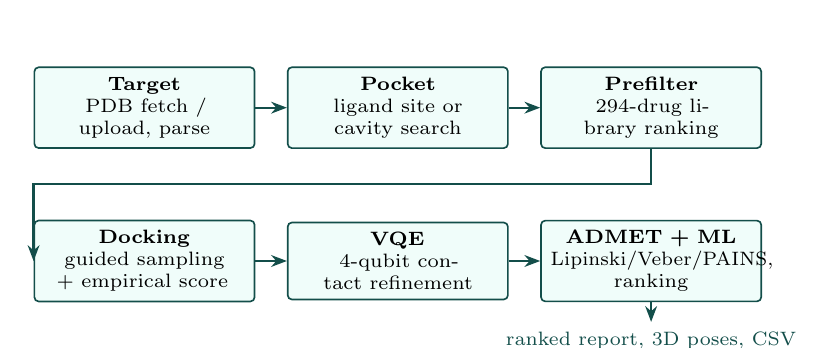
\begin{tikzpicture}[
    node distance=2.5mm and 4mm,
    box/.style={draw=prespdf, semithick, rounded corners=1.5pt, fill=presbox,
                text width=2.55cm, align=center, font=\scriptsize, inner sep=3.5pt, minimum height=8.5mm},
    arr/.style={-{Stealth[length=2mm]}, thick, color=prespdf}
  ]
  \node[box] (a) {\textbf{Target}\\\scriptsize PDB fetch / upload, parse};
  \node[box, right=of a] (b) {\textbf{Pocket}\\\scriptsize ligand site or cavity search};
  \node[box, right=of b] (c) {\textbf{Prefilter}\\\scriptsize 294-drug library ranking};
  \node[box, below=9mm of a] (d) {\textbf{Docking}\\\scriptsize guided sampling + empirical score};
  \node[box, right=of d] (e) {\textbf{VQE}\\\scriptsize 4-qubit contact refinement};
  \node[box, right=of e] (f) {\textbf{ADMET + ML}\\\scriptsize Lipinski/Veber/PAINS, ranking};
  \draw[arr] (a) -- (b);
  \draw[arr] (b) -- (c);
  \draw[arr] (c.south) |- ++(0,-4.5mm) -| (d.west);
  \draw[arr] (d) -- (e);
  \draw[arr] (e) -- (f);
  \node[below=2.5mm of f, font=\scriptsize, text=prespdf] (rep) {ranked report, 3D poses, CSV};
  \draw[arr] (f) -- (rep);
\end{tikzpicture}
\caption{Q-Pharm screening pipeline. Every stage reports progress to the
web console; all artefacts (poses, structures, CSV export) are served from the job
directory.}
\label{fig:pipeline}
\end{figure}

\subsection{Target acquisition and pocket detection}

Structures are fetched from the RCSB PDB over HTTPS or accepted as uploads. The parser
keeps the first model, resolves alternate locations, maps modified residues to their
parents (e.g.\ selenomethionine to methionine) and classifies every \texttt{HETATM}
group. Pocket definition uses two strategies in order of preference. If a drug-like
co-crystal ligand (6--70 heavy atoms, excluding waters, ions, buffers and glycans) is
present, the pocket comprises all protein residues with an atom within 6.5~\AA{} of it;
for curated targets the reference ligand is pinned explicitly (for example the
remediated inhibitor code PJE for the N3 inhibitor in 6LU7). Otherwise, a
LIGSITE-style detector samples a 1.4~\AA{} voxel grid, keeps voxels at least 3~\AA{}
from any protein atom but inside the protein's convex hull, and flood-fills connected
cavity clusters, selecting the largest.

Both receptor and ligand atoms are typed into four pharmacophore classes: hydrogen-bond
donors, hydrogen-bond acceptors, hydrophobic atoms and aromatic ring centroids. Receptor
typing uses residue- and atom-name rules; ligand typing uses RDKit SMARTS patterns.

\subsection{Docking engine}
\label{sec:docking}

\textbf{Conformers.} RDKit ETKDGv3 generates 3--6 conformers per drug (adaptive to
molecule size), relaxed with MMFF94 (UFF fallback); Gasteiger charges provide ligand
partial charges.

\textbf{Placement.} Docking is rigid-receptor with rigid-body sampling. A lattice of
\emph{cavity anchors}---points inside the pocket sphere that are themselves at least
3~\AA{} from every receptor atom---guarantees that most sampled placements begin
geometrically feasible. Half of the placements receive pharmacophore seeding: one ligand
donor or acceptor is placed at the ideal 2.85~\AA{} hydrogen-bond distance from a
complementary pocket atom, with a random orientation about that axis; the remainder use
uniform random rotations about anchors. A KD-tree clash filter against the full protein
rejects poses with any atom pair below 2.35~\AA.

\textbf{Scoring.} Poses are evaluated with an empirical function whose terms and weights
are
\begin{equation}
\begin{aligned}
E = \; & 8.0\!\sum_{d_i<2.55}(2.55-d_i)^2
        - 0.062\!\sum \mathrm{e}^{-(d-3.8)^2/0.8}\\
       & - 2.6\!\sum_{\text{D}\cdots\text{A}}\!\mathrm{e}^{-(d-2.85)^2/0.2}
        - 0.105\!\sum_{\text{hh}}\!\mathrm{e}^{-(d-4.0)^2/0.9}\\
       & + 83\!\sum_{i,j}\frac{q_i q_j}{4d_{ij}^2}
        - 1.2\,N_{\pi\text{-stack}} + 0.35\,N_{\text{rot}},
\end{aligned}
\label{eq:score}
\end{equation}
where the first term penalizes steric clashes, followed by van der Waals attraction,
hydrogen bonds (donor--acceptor pairs in 2.3--3.8~\AA), hydrophobic contacts
(3.2--5.6~\AA), a distance-dependent electrostatic term with formal receptor charges,
aromatic stacking, and a rotatable-bond entropy penalty (all in kcal~mol$^{-1}$-like
units).

\textbf{Refinement.} The best placement is polished by 90 greedy-or-Metropolis moves
alternating random perturbations with \emph{snap moves} that translate a ligand
donor/acceptor onto the ideal hydrogen-bond distance from a complementary pocket atom.
Improvements are always accepted; small regressions are accepted with a decreasing
temperature to escape single-hydrogen-bond basins. Ligands for which no placement is
clash-free are retained with their least-clashing pose and flagged \emph{no-fit}; a
0.3$\times$ composite multiplier prevents steric incompatibility from being outvoted by
favourable contact terms.

\subsection{Quantum refinement}
\label{sec:quantum}

Classical scores treat electrons implicitly, yet binding is an electronic event: charge
transfer across a hydrogen bond. For each top-ranked pose, Q-Pharm extracts the strongest
polar contact---the shortest ligand donor$\cdots$acceptor or acceptor$\cdots$donor pair
within 3.6~\AA---and models it as a two-site, two-orbital Hubbard dimer with modes
$(1\uparrow, 2\uparrow, 1\downarrow, 2\downarrow)$:
\begin{equation}
\begin{aligned}
H = \; & -t \sum_\sigma \left(c^\dagger_{1\sigma} c_{2\sigma} + \text{h.c.}\right)
       + U \sum_\sigma n_{1\sigma} n_{1\bar\sigma} \\
       & + \frac{\delta}{2} \sum_\sigma (n_{1\sigma} - n_{2\sigma}),
\end{aligned}
\label{eq:hubbard}
\end{equation}
with distance- and chemistry-derived parameters
\begin{equation}
t = t_0\, e^{-(d - 2.9\text{\AA})/0.9}, \qquad
\delta = 1.4\,(\chi_{\text{lig}} - \chi_{\text{prot}}),
\end{equation}
where $t_0 = 0.045$~E$_h$, $U = 0.28$~E$_h$ and $\chi$ denotes Pauling electronegativity.
The four-mode Hamiltonian is mapped exactly to four qubits (Jordan--Wigner
\cite{jordanwigner1928}; verified numerically against the fermionic matrix in the test
suite) and expanded in the Pauli basis (15--16 terms after the particle-number penalty
below).

The ground state is found with a VQE \cite{peruzzo2014}: a hardware-efficient
$R_y$ ansatz (depth 2, twelve parameters) is optimized by L-BFGS-B with \emph{exact
parameter-shift gradients} and two random restarts. Because the ansatz does not conserve
particle number, a penalty $\lambda (N-2)^2$ with $\lambda = 0.6$~E$_h$ pins the
variational state to the physical two-electron sector---a standard technique when
particle-number symmetry is not built into the circuit. The interaction energy
\begin{equation}
\de = E_{\text{coupled}}(t) - E_{\text{decoupled}}(t{=}0)
\end{equation}
quantifies charge-transfer stabilization; negative values indicate that the contact
benefits from the electronic channel. All simulations run on Qiskit's statevector
backend \cite{qiskit2024}; each refined contact costs approximately four seconds on a
laptop CPU.

We emphasize the intended reading of this stage: it is a \emph{proof-of-concept
refinement} on an effective model with phenomenological parameters, not an ab initio
electronic-structure calculation. Its purpose is to exercise, end-to-end and
openly, the architecture proposed for near-term quantum advantage in drug discovery
\cite{cao2019,li2024}; replacing the contact-parameterization step with an active-space
Hamiltonian from ab initio methods would change nothing else in the loop.

\subsection{ADMET profiling and machine-learning re-ranking}

Each docked compound is profiled with the standard filter cascade: Lipinski Rule of 5
violations \cite{lipinski1997}; Veber oral-bioavailability rules \cite{veber2002};
PAINS and Brenk structural alerts via RDKit's filter catalogue \cite{baell2010}; and
ESOL estimated solubility \cite{delaney2004},
\begin{equation}
\log S = 0.16 - 0.63\,\mathrm{cLog}P - 0.0062\,\mathrm{MW} + 0.066\,\mathrm{rotB} - 0.74\,\mathrm{AP}.
\end{equation}
A logistic-regression drug-likeness prior over eleven RDKit descriptors is trained at
build time on the drug library itself (positives) against curated non-drug
chemicals---industrial solvents, dyes, pesticides and alkylating toxophores
(negatives). It is a transparent illustration of the re-ranking stage rather than a
production QSAR ensemble, and its predictions are displayed as such in the console.

\subsection{Composite ranking}

All signals are fused with fixed, published weights:
\begin{equation}
S = 0.55\,\widehat{E}_{\text{dock}} + 0.20\,A + 0.15\,Q + 0.10\,M,
\label{eq:composite}
\end{equation}
where $\widehat{E}_{\text{dock}}$ is the min--max-normalized docking score (inverted so
that stronger binders score higher), $A$ the ADMET score, $Q$ the normalized quantum
stabilization and $M$ the ML prior. Ligands flagged \emph{no-fit} receive a
$0.3\times$ multiplier. Every candidate exposes all four components in the console.

% ---------------------- 4 implementation ---------------------- %
\section{Implementation}

The backend is Python 3.11 with FastAPI, RDKit 2026.03, NumPy/SciPy and Qiskit 2.5
\cite{rdkit,qiskit2024}; the frontend is React 18 with Vite, Tailwind CSS and 3Dmol.js
\cite{rego2015}. The drug library (294 compounds spanning antiviral, antibacterial,
antiparasitic, central-nervous-system, cardiovascular, oncology and anti-inflammatory
classes; 38 with documented repurposing histories) is resolved from PubChem by name or
CID, validated with RDKit and stored as canonical SMILES; a deterministic build script
reconstructs all data artefacts and retrains the ML model. Ten curated targets were
verified against RCSB at build time with explicit reference ligands (for example PJE
for 6LU7, F86 for remdesivir monophosphate in the polymerase structure 7BV2, and the
oseltamivir code G39 in neuraminidase 2HU4). Docked poses are exported in the original
PDB coordinate frame, so poses overlay the receptor without alignment. The API exposes
job submission, progress polling, structure and pose files, CSV export and an OpenAPI
schema; finished screenings are addressable by permalink. The complete system is 61
tracked files, MIT-licensed.

% ---------------------- 5 results ---------------------- %
\section{Validation and results}
\label{sec:results}

\subsection{Correctness of the quantum module}

The half-filled Hubbard dimer admits the analytic ground state
$E = U/2 - \sqrt{(U/2)^2 + 4t^2}$ at zero site offset. The fermionic construction
reproduces this expression to $10^{-9}$~E$_h$ across the hopping range, and the VQE
converges to the same curve: across six hopping values spanning an order of magnitude,
the maximum deviation between VQE and the analytic energy is
$4.8\times10^{-12}$~E$_h$ (Figure~\ref{fig:vqe}), using twelve variational parameters
and two restarts. This confirms the three correctness links of the quantum chain---the
fermionic Hamiltonian, its qubit mapping and the variational solver.

\begin{figure}[t]
\centering
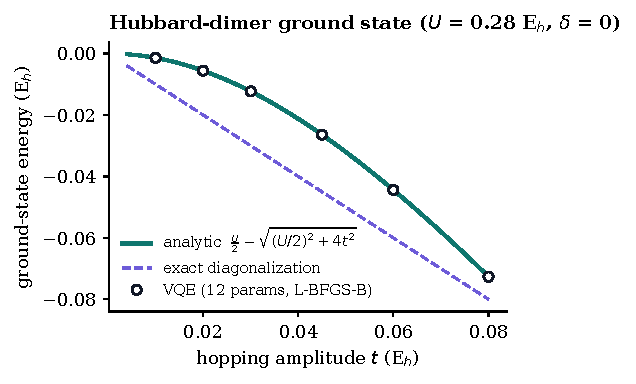
\includegraphics[width=\columnwidth]{figures/fig_vqe.pdf}
\caption{Hubbard-dimer ground state used by the quantum-refinement stage. The analytic
half-filled solution (solid) and exact diagonalization of the four-qubit Hamiltonian
(dashed) coincide; live VQE runs (circles, computed with the released implementation)
land on the same curve to within $4.8\times10^{-12}$~E$_h$.}
\label{fig:vqe}
\end{figure}

\subsection{End-to-end screening of SARS-CoV-2 M$^{pro}$}

We screened the default 60-drug prefiltered library against PDB~6LU7, the crystal
structure of the SARS-CoV-2 main protease in complex with inhibitor N3 \cite{jin2020}.

\textbf{Pocket reproduction.} The ligand-anchored pocket detector selected the
co-crystallized inhibitor site and recovered 22 residues---His41 and Cys145 (the
catalytic dyad), Met49, Met165, Glu166, Gln189, Asn142, Gly143 and neighbours---matching
the experimentally established active site. The pocket's chemical inventory (21 donors,
26 acceptors, 55 hydrophobic atoms, 4 aromatic rings) drives the subsequent typing and
placement stages.

\textbf{Screening outcome.} All 60 selected drugs were docked (18{,}000 sampled
placements; 362~s total on a consumer laptop, of which the eight VQE refinements
contributed roughly 30~s). Table~\ref{tab:hits} lists the top ten by composite score;
Figure~\ref{fig:screening} visualizes the same data. The top-ranked hit, amoxicillin,
makes seven recorded interactions including four hydrogen bonds to Asn142, Thr26 and
Leu4 at 2.66--3.11~\AA, with a VQE contact stabilization of $-0.50$~eV at an
S$\cdots$N distance of 2.66~\AA. Nucleoside-antiviral pharmacophores rank prominently
(entecavir, sofosbuvir, molnupiravir, ribavirin), consistent with the target's
preference for peptidomimetic and polar inhibitors; the largest macromolecules
(vancomycin, daptomycin) are correctly flagged \emph{no-fit} despite locally attractive
contact scores, demonstrating that the steric guard behaves as designed.

\begin{table*}[t]
\centering
\caption{Top ten candidates from the 60-drug screening of SARS-CoV-2 M$^{pro}$
(PDB~6LU7). $\dg$ is the empirical docking score of Equation~\ref{eq:score};
$\de$ is the VQE interaction energy of the strongest polar contact (dash: pose not among
the quantum-refined top eight); $A$ is the ADMET grade (A best to D worst); $S$ is the
composite of Equation~\ref{eq:composite}. Values are computational estimates, not
measurements.}
\label{tab:hits}
\footnotesize
\begin{tabular*}{\textwidth}{@{\extracolsep{\fill}} c l l r r c r l}
\toprule
Rank & Compound & Class & $\dg$ (kcal/mol) & $\de$ (eV) & $A$ & $S$ & Contacts of best pose \\
\midrule
1  & Amoxicillin   & $\beta$-lactam antibiotic & $-12.9$ & $-0.50$ & A & 0.700 & 4 H-bonds (Asn142, Thr26) \\
2  & Mannitol      & Osmotic diuretic          & $-8.6$  & $-1.07$ & A & 0.670 & polyol H-bond network \\
3  & Zanamivir     & Neuraminidase inhib.      & $-8.6$  & $-1.57$ & D & 0.639 & glycerol-chain H-bonds \\
4  & Sulfasalazine & Aminosalicylate           & $-14.6$ & $-0.51$ & C & 0.620 & sulfonamide + azo contacts \\
5  & Entecavir     & Nucleoside analog (HBV)   & $-7.6$  & $-0.44$ & A & 0.572 & exocyclic amine H-bonds \\
6  & Ceftriaxone   & Cephalosporin             & $-9.8$  & $-1.03$ & D & 0.558 & O14$\cdots$N 2.66~\AA\ contact \\
7  & Sofosbuvir    & NS5B inhibitor (HCV)      & $-8.2$  & $-0.61$ & C & 0.535 & phosphoramidate contacts \\
8  & Molnupiravir  & Nucleoside analog         & $-7.5$  & ---     & B & 0.529 & cytidine-analog H-bonds \\
9  & Ribavirin     & Broad-spectrum antiviral  & $-5.5$  & ---     & A & 0.525 & base-mimic H-bonds \\
10 & Dabigatran    & Thrombin inhibitor        & $-8.6$  & $-0.44$ & C & 0.518 & benzimidazole stacking \\
\bottomrule
\end{tabular*}
\end{table*}

\begin{figure*}[t]
\centering
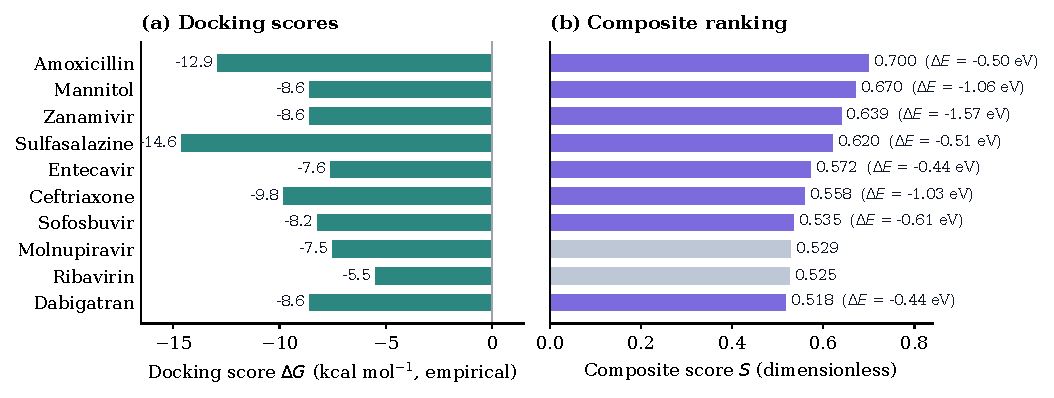
\includegraphics[width=0.98\textwidth]{figures/fig_screening.pdf}
\caption{Real output of the released pipeline for the 60-drug screen of SARS-CoV-2
M$^{pro}$ (PDB~6LU7). (a) Empirical docking scores of the top ten candidates by
composite rank; more negative is better. (b) Composite scores; violet bars indicate
candidates whose strongest contact was refined by the four-qubit VQE (with the resulting
charge-transfer stabilization $\de$), grey bars were not among the quantum-refined top
eight.}
\label{fig:screening}
\end{figure*}

\textbf{Negative controls.} Molecules that physically cannot occupy the pocket are
handled transparently: vancomycin (101 heavy atoms) and daptomycin (115) return their
least-clashing poses with unfavourable net scores and the \emph{no-fit} flag, and are
excluded from quantum refinement. In an earlier build without full-protein clash
checking, such compounds could rank spuriously high; the guard was added and is covered
by regression tests.

\subsection{Performance}

On a consumer laptop (Windows 11, no GPU), the 60-drug screen completes in
$362\pm10$~s: pocket detection and prefiltering take under 3~s, docking averages
$\sim$5~s per drug (dominated by conformer generation for macromolecules), and each VQE
refinement adds $\sim$4~s. The Fast preset (25 drugs) completes in roughly
2.5--3~minutes. Memory use is modest; the system runs entirely from simulators and
public databases with no proprietary dependencies.

% ---------------------- 6 limitations ---------------------- %
\section{Limitations and discussion}

\textbf{Docking realism.} The receptor is rigid, waters and protonation states are not
modelled, and side-chain flexibility is absent. The scoring function is empirical and
calibrated only against pocket geometry and known complex chemistry; absolute scores
should be compared \emph{within} a run, never interpreted as free energies.

\textbf{Quantum layer.} The Hubbard-dimer refinement uses phenomenological parameters
and a statevector simulator. It demonstrates the hybrid architecture honestly and
validates it numerically, but it does not produce ab initio energetics. We consider this
the correct scope for an open reference implementation; the API contract isolates the
parameterization so that an active-space Hamiltonian can replace it without touching the
pipeline.

\textbf{ADMET.} The ML prior is trained on a small curated set and saturates for very
drug-like molecules; it discriminates gross non-drug chemistry reliably but should not
be read as a pharmacokinetics prediction.

\textbf{Library coverage.} 294 curated compounds is a deliberate, license-clean subset,
not the full DrugBank; the build script is designed for extension.

\textbf{Intended use.} Q-Pharm ranks hypotheses. Any candidate of interest requires
literature follow-up and experimental validation before anyone should draw biological or
medical conclusions from it.

% ---------------------- 7 conclusion ---------------------- %
\section{Conclusion and availability}

Q-Pharm shows that a meaningful drug-repurposing screen---structure acquisition, pocket
detection, guided docking, a four-qubit VQE refinement, ADMET filtering and an
interpretable composite ranking---can now be assembled entirely from open components and
run on a laptop in minutes. The quantum stage is implemented as real, validated
hybrid quantum--classical computation on an effective model, providing a reproducible
scaffold that ab initio methods can upgrade in place. The system is available under the
MIT license at \url{https://github.com/Shreyasderaje/q-pharm}, with a browser console,
documented API, deterministic data builds and a test suite covering every module,
including the analytic correctness of the quantum chain.

\subsection*{Acknowledgements}
The author thanks the open-source scientific Python and quantum-computing communities,
and the RCSB PDB and PubChem teams, whose public data services this project builds on.

% ---------------------- references ---------------------- %
\begin{thebibliography}{99}
\footnotesize
\setlength{\itemsep}{1.5pt}

\bibitem{pushpakom2019} Pushpakom, S. et al. Drug repurposing: progress, challenges and
recommendations. \emph{Nat. Rev. Drug Discov.} \textbf{18}, 41--58 (2019).

\bibitem{beigel2020} Beigel, J.~H. et al. Remdesivir for the treatment of Covid-19 ---
final report. \emph{N. Engl. J. Med.} \textbf{383}, 1813--1826 (2020).

\bibitem{jin2020} Jin, Z. et al. Structure of M$^{\text{pro}}$ from SARS-CoV-2 and
discovery of its inhibitors. \emph{Nature} \textbf{582}, 289--293 (2020).

\bibitem{yin2020} Yin, W. et al. Structural basis for inhibition of the RNA-dependent
RNA polymerase from SARS-CoV-2 by remdesivir. \emph{Science} \textbf{368},
1499--1504 (2020).

\bibitem{bohm1992} B\"ohm, H.-J. The computer program LUDI: a new method for the de novo
design of enzyme inhibitors. \emph{J. Comput. Aided Mol. Des.} \textbf{6}, 61--78 (1992).

\bibitem{lipinski1997} Lipinski, C.~A., Lombardo, F., Dominy, B.~W. \& Feeney, P.~J.
Experimental and computational approaches to estimate solubility and permeability in
drug discovery and development settings. \emph{Adv. Drug Deliv. Rev.} \textbf{23},
3--25 (1997).

\bibitem{veber2002} Veber, D.~F. et al. Molecular properties that influence the oral
bioavailability of drug candidates. \emph{J. Med. Chem.} \textbf{45}, 2615--2623 (2002).

\bibitem{baell2010} Baell, J.~B. \& Holloway, G.~A. New substructure filters for removal
of pan assay interference compounds (PAINS) from screening libraries. \emph{J. Med.
Chem.} \textbf{53}, 2719--2740 (2010).

\bibitem{delaney2004} Delaney, J.~S. ESOL: estimating aqueous solubility directly from
molecular structure. \emph{J. Chem. Inf. Comput. Sci.} \textbf{44}, 1000--1005 (2004).

\bibitem{peruzzo2014} Peruzzo, A. et al. A variational eigenvalue solver on a photonic
quantum processor. \emph{Nat. Commun.} \textbf{5}, 4213 (2014).

\bibitem{kandala2017} Kandala, A. et al. Hardware-efficient variational quantum
eigensolver for small molecules and quantum magnets. \emph{Nature} \textbf{549},
242--246 (2017).

\bibitem{cao2019} Cao, Y., Romero, J., McClean, J.~P., Hastings, E., Babbush, R. \&
Aspuru-Guzik, A. Quantum chemistry in the age of quantum computing. \emph{Chem. Rev.}
\textbf{119}, 10856--10915 (2019).

\bibitem{jordanwigner1928} Jordan, P. \& Wigner, E. \"Uber das Paulische
\"Aquivalenzverbot. \emph{Z. Phys.} \textbf{47}, 631--651 (1928).

\bibitem{li2024} Li, J. et al. A hybrid quantum computing pipeline for real world drug
discovery. \emph{Sci. Rep.} \textbf{14} (2024).

\bibitem{berman2000} Berman, H.~M. et al. The Protein Data Bank. \emph{Nucleic Acids
Res.} \textbf{28}, 235--242 (2000).

\bibitem{kim2023} Kim, S. et al. PubChem 2023 update. \emph{Nucleic Acids Res.}
\textbf{51}, D523--D531 (2023).

\bibitem{rego2015} Rego, N. \& Koes, D. 3Dmol.js: molecular visualization with WebGL.
\emph{Bioinformatics} \textbf{31}, 1322--1324 (2015).

\bibitem{rdkit} Landrum, G. et al. RDKit: open-source cheminformatics software.
\url{https://www.rdkit.org} (accessed October 2026).

\bibitem{qiskit2024} Javadi-Abhari, A. et al. Quantum computing with Qiskit.
\emph{arXiv:2405.08810} (2024).

\end{thebibliography}

\end{document}
